% // ============================================================================
%//
%// Copyright (c) 1999 The CGAL Consortium
%//
%// This software and related documentation is part of an INTERNAL release
%// of the Computational Geometry Algorithms Library (CGAL). It is not
%// intended for general use.
%//
%// ----------------------------------------------------------------------------
%//
%// release       :
%// release_date  :
%//
%// file          : /doc_tex/basic/Triangulation3/Triangulation3.tex
%// revision      : $Revision$
%//
%// author(s)     : Monique Teillaud <Monique.Teillaud@sophia.inria.fr>
%//
%// coordinator   : INRIA Sophia Antipolis (Mariette Yvinec <Mariette.Yvinec@sophia.inria.fr>)
%//
%//============================================================================
\chapter{Triangulation in 3D}
\label{chapter-Triangulation3}
\begin{ccTexOnly}
\vspace*{-2cm}
\includegraphics{grille.eps} \hspace*{2cm} 
\includegraphics{sphere.eps} 
\end{ccTexOnly}
\begin{ccHtmlOnly}
<img border=0 src="./sphere.gif" align=center>
\end{ccHtmlOnly}
\section{Introduction}
\label{Triangulation3-sec-intro}
\subsection{Definition}
\label{Triangulation3-sec-def}
A three-dimensional triangulation is a three-dimensional simplicial
complex, pure connected and without singularities. (See
\cite{by-ag-98} or Chapter~\ref{I1_Chapter_Triangulations}.) Its
cells ($3$-faces) are such that two cells either do not intersect or
share a common facet ($2$-face), edge ($1$-face) or vertex ($0$-face).

The basic 3D-triangulation class of \cgal\ is primarily designed to
represent the triangulations of a set of points $A$ in $\R^3$.  It can
be viewed as a partition of the convex hull of {$A$} into tetrahedra
whose vertices are the points of {$A$}.  Together with the unbounded
cell having the convex hull boundary as its frontier, the triangulation
forms a partition of $\R^3$.

In order to deal
only with tetrahedra, which is convenient for many applications, the
unbounded cell can be subdivided into tetrahedra by considering that
each convex hull facet is incident to an \ccc{infinite cell} having as
fourth vertex an auxiliary vertex called the \ccc{infinite vertex}.  In
that way, each facet is incident to exactly two cells and special cases
at the boundary of the convex hull are simple to deal with.

The class \ccc{Triangulation_3<Traits,Tds>} of \cgal\ implements this
point of view and therefore considers the triangulation of the set
of points as a set of finite and infinite tetrahedra.  Notice that the
infinite vertex has no significant coordinates and that no
geometric predicate can be applied on it.

A triangulation is a collection of vertices and cells that are linked
together through incidence and adjacency relations. Each cell gives
access to its four incident vertices and to its four adjacent
cells. Each vertex gives access to one of its incident cells.

The four vertices of a cell are indexed with 0, 1, 2 and 3 in positive
orientation, the positive orientation being defined by the orientation
of the underlying Euclidean space $\R^3$. The neighbors of a cell are also
indexed with 0, 1, 2, 3 in such a way that the neighbor indexed by $i$
is opposite to the vertex with the same index. See
Figure~\ref{Triangulation3-fig-orient}.

\begin{figure}[htbp]
\begin{ccTexOnly}
\begin{center} 
\includegraphics{orient.eps} 
\end{center}
\end{ccTexOnly}
\caption{Orientation of a cell (3-dimensional case).
\label{Triangulation3-fig-orient}}
\begin{ccHtmlOnly}
<CENTER>
<img border=0 src="./orient.gif" align=center alt="Orientation of a cell 
(3-dimensional case)">
</CENTER>
\end{ccHtmlOnly}
\end{figure} 

As in the underlying combinatorial triangulation (see
Chapter~\ref{chapter-TDS3}), edges ($1$-faces) and facets ($2$-faces)
are not explicitly 
represented: a facet is given by a cell and an index (the facet
\ccc{i} of a cell \ccc{c} is the facet of \ccc{c} that is opposite to
the vertex with index \ccc{i}) and an edge is given by a cell and two
indices (the edge \ccc{(i,j)} of a cell \ccc{c} is the edge whose
endpoints are the vertices of \ccc{c} with indices \ccc{i} and
\ccc{j}). See Figure~\ref{TDS3-fig-repres}.  

\subsection{Degenerate Dimensions}
\label{Triangulation3-sec-degen_dim}

The class \ccc{Triangulation_3<Traits,Tds>} can also deal with
triangulations whose dimension is less than~3. A triangulation of a
set of points in $\R^d$ covers the whole space $\R^d$ and consists of
cells having $d+1$ vertices: some of them are infinite, they are
obtained by linking the additional infinite vertex to each facet of
the convex hull of the points.
\begin{itemize}
\item {} \emph{dimension 2:} when a triangulation only contains
coplanar points (which is the case when there are only three points), 
it consists of triangular faces.
\item {} \emph{dimension 1:} the triangulation contains only collinear 
points (which is the case when there are only two points), it consists
of edges.
\item {} \emph{dimension 0:} the triangulation contains only one
finite point.
\item {} \emph{dimension -1:} this is a convention to handle the case
when the only vertex of the triangulation is the infinite one.
\end{itemize} 

The same cell class is used in all cases: triangular faces in
2D can be considered as degenerate cells, having only three vertices
(resp. neighbors)
numbered $(0,1,2)$, and one $NULL$ vertex (resp. neighbor);
edges in 1D have only two vertices (resp. neighbors) numbered $0$ and $1$. 

The implicit representation of facets (resp. edges) still holds
for degenerate dimensions (\textit{i.e.}dimensions $<3$) : in
dimension~2, each cell has only one facet of index 3, and 3 edges
$(0,1)$, $(1,2)$ and $(2,0)$; in dimension~1, each cell has one edge
$(0,1)$.  

\subsection{Validity}
\label{Triangulation3-sec-Valid}

A triangulation of $\R^3$ is said to be \ccc{locally valid} iff

{\bf (a)-(b)} Its underlying combinatorial graph, the triangulation
data structure, is \ccc{locally valid} 
(see Section~\ref{TDS3-sec-Valid} of Chapter~\ref{chapter-TDS3})\\
{\bf (c)} Any cell has its vertices ordered according to positive
orientation. See Figure~\ref{Triangulation3-fig-orient}.

When the triangulation is degenerated into a triangulation of
dimension~2, the  geometric validity reduces to:

{\bf (c-2D)} For any two adjacent triangles $(u,v,w_1)$ and $(u,v,w_2)$ with
common edge $(u,v)$, $w_1$ and $w_2$ lie on opposite sides of $(u,v)$
in the plane.

When all the points are collinear, this condition becomes:

{\bf (c-1D)} For any two adjacent edges $(u,v)$ and $(v,w)$, $u$ and
$w$ lie on opposite sides of the common vertex $v$ on the line.

The \ccc{is_valid()} method provided by \cgal\ checks the local
validity of a given triangulation. This does not always
ensure global validity \cite{mnssssu-cgpvg-96,dlpt-ccpps-98} but it is 
sufficient for practical cases.

\section{Software Design}
\label{Triangulation3-sec-design}

The class \ccc{Triangulation_3<Traits,Tds>} is designed to be used as 
a layer upon a 3D-triangulation data structure as presented in 
Section~\ref{TDS3-sec-design} of Chapter~\ref{chapter-TDS3}.
It provides high level geometric operations such as location of a point
in the triangulation and insertion of a point, and is responsible for
the geometric validity. This class is parameterized by two classes:
\begin{itemize}
\item {} the \textbf{geometric traits} class, where the user can
specify the type of points to use as well as the elementary
operations on them (predicates,\ldots). The concept of such a class is
described in Section~\ref{Triangulation3-sec-concept-Traits} and a
model is provided by \cgal\ (see
Section~\ref{Triangulation3-sec-class-Traits}).
\item {} the \textbf{triangulation data structure} class of the middle level, 
described in Chapter~\ref{chapter-TDS3}.
\end{itemize}	

Delaunay triangulations as well as hierarchical Delaunay triangulations
\cite{d-iirdt-98} are also implemented in the package: 
\ccc{Delaunay_triangulation_3<Traits,Tds>} inherits from 
\ccc{Triangulation_3<Traits,Tds>} and 
\ccc{Delaunay_hierarchic_triangulation_3<Traits,Tds>} inherits from 
\ccc{Delaunay_triangulation_3<Traits,Tds>}. \textit{(Hierarchical
Delaunay triangulations are not yet implemented.)} 

\ccc{Triangulation_3<Traits,Tds>} derives from
\ccc{Triangulation_utils_3<Traits,Tds>}, which defines a set of tools
working on the indices of vertices in cells (see
Section~\ref{Triangulation3-sec-class-Utils}). 

\section{Examples}
\label{Triangulation3-sec-examples}
This example shows the incremental construction of a 3D triangulation, 
the location of a point, and how to manipulate elementary operations
on indices in a cell.

\begin{verbatim}
#include <CGAL/basic.h>

#include <iostream>

#include <list>
#include <vector>

#include <CGAL/Cartesian.h>

#include <CGAL/Triangulation_cell_base_3.h>
#include <CGAL/Triangulation_vertex_base_3.h>
#include <CGAL/Triangulation_data_structure_3.h>
#include <CGAL/Triangulation_geom_traits_3.h>
#include <CGAL/Triangulation_3.h>

typedef CGAL::Cartesian<double>  Rep;

typedef CGAL::Triangulation_geom_traits_3<Rep> Gt;
typedef CGAL::Triangulation_vertex_base_3<Gt> Vb;
typedef CGAL::Triangulation_cell_base_3<Gt>  Cb;

typedef CGAL::Triangulation_data_structure_3<Vb,Cb> TDS;
typedef CGAL::Triangulation_3<Gt,TDS> Triangulation;

typedef typename Triangulation::Cell_handle Cell_handle;
typedef typename Triangulation::Vertex_handle Vertex_handle;
typedef typename Triangulation::Locate_type Locate_type;

typedef Gt::Point Point;

int main(int argc, char* argv[])
{

  Triangulation T;

  // insertion from a list :
  std::list<Point> L;
  L.push_front(Point(0,0,0));
  L.push_front(Point(1,0,0));
  L.push_front(Point(0,1,0));

  int n = T.insert(L.begin(), L.end());

  // insertion from a vector :
  std::vector<Point> V(3);
  V[0] = Point(0,0,1);
  V[1] = Point(1,1,1);
  V[2] = Point(2,2,2);

  n = n + T.insert(V.begin(), V.end());

  // 6 points have been inserted :
  assert( n == 6 );

  // checking validity of T :
  assert( T.is_valid(false) );

  Locate_type lt;
  int li, lj;
  Point p(0,0,0);
  Cell_handle c = T.locate(p, lt, li, lj);
  // p is the vertex of c of index li :
  assert( lt == Triangulation::VERTEX );
  assert(  c->vertex(li)->point() == p );

  Vertex_handle v = c->vertex( (li+1)&3 );
  // v is another vertex of c
  Cell_handle nc = c->neighbor(li);
  // nc = neighbor of c opposite to the vertex associated with p
  // nc must have vertex v :
  int nli;
  assert( nc->has_vertex( v, nli ) );
  // nli is the index of v in nc

  std::ofstream oFileT("output",ios::out);
  // writing file output; 
  oFileT << T; 

  return 0;
}
\end{verbatim}

\clearpage


%\section{A Class of Tools \protect\ccc{Triangulation_utils_3}} 
\section{A Class of Tools}
\label{Triangulation3-sec-class-Utils}

\begin{ccClass}{Triangulation_utils_3}
This class defines operations on the indices of vertices and neighbors 
within a cell. These operations are used in \ccc{Triangulation_3.h},
\ccc{Triangulation_data_structure_3.h},
\ccc{Triangulation_ds_cell_3.h},
\ccc{Triangulation_ds_circulators_3.h}. These classes inherit from
\ccClassName\ so that they can use its methods.

\ccThree{unsigned int}{ccw(unsigned int i)toto}{}

\ccFunction{unsigned int next_around_edge(unsigned int i, 
				    unsigned int j) const;}
{In dimension~3, index of the neighbor \ccc{n} that is next to the current cell,
when turning positively around an oriented edge whose endpoints are
indexed \ccc{i} and \ccc{j}. According to the usual numbering of
vertices and neighbors in a given cell, it is also the index of the vertex 
opposite to this neighbor \ccc{n}. (see Figure~\ref{Triangulation3-fig-utils}).
\ccPrecond{\ccc{( i < 4 ) && ( j < 4 ) && ( i != j )}.}}

\ccFunction{unsigned int ccw(unsigned int i) const;}
{Has a meaning only in dimension~2.\\
 Computes the index of the vertex that is next to the vertex numbered
\ccc{i} in counterclockwise direction. (see
Figure~\ref{Triangulation3-fig-utils}).  
\ccPrecond{\ccc{i<3}.}}

\ccFunction{unsigned int cw(unsigned int i) const;}
{Same for clockwise.}

\begin{figure}[htbp]
\begin{ccTexOnly}
\begin{center} 
\includegraphics{utils.eps} 
\end{center}
\end{ccTexOnly}
\caption{Operations on indices.
\label{Triangulation3-fig-utils}}
\begin{ccHtmlOnly}
<CENTER>
<img border=0 src="./utils.gif" align=center alt="Operations on indices">
</CENTER>
\end{ccHtmlOnly}
\end{figure} 

\end{ccClass}

%\section{The Triangulation Class \protect\ccc{Triangulation_3<Traits,Tds>} }
\section{Basic Triangulation}

\ccDefinition

\begin{ccClassTemplate}{Triangulation_3<Traits,Tds>}
The \ccClassTemplateName\ expects a model of a \ccc{geometric traits
class} as its first template argument and a model of a \ccc{triangulation data
structure} as its second argument. The requirements and defaults for these
classes are described in Sections~\ref{Triangulation3-sec-concept-Traits} 
and~\ref{Triangulation3-sec-class-Traits}.

\ccInclude{CGAL/Triangulation_3.h}

\ccInheritsFrom{\ccc{Triangulation_utils_3}}
(see Section~\ref{Triangulation3-sec-class-Utils})

\ccTypes
The class \ccClassTemplateName\ defines the following types:
\ccThree{typedef Traits::Tetrahedron Tetrahedron;}{Tetrahedron}{}
\ccThreeToTwo

\ccTypedef{typedef Traits::Point Point;}{}
\ccGlue
\ccTypedef{typedef Traits::Segment Segment;}{}
\ccGlue
\ccTypedef{typedef Traits::Triangle Triangle;}{}
\ccGlue
\ccTypedef{typedef Traits::Tetrahedron Tetrahedron;}{}

The following types represent $k$-faces for $k\in\{0,1,2,3\}$. Edges
($1$-faces) and facets ($2$-faces) are not explicitly represented and
thus there are no corresponding classes (see
Sections~\ref{Triangulation3-sec-degen_dim} and
~\ref{Triangulation3-sec-def}). The functionalities of the 
vertex and cell classes ($0$- and $3$-faces) are described in
Sections~\ref{Triangulation3-sec-class-Vertex}
and~\ref{Triangulation3-sec-class-Cell}.

\ccNestedType{Vertex}{Vertex type}
\ccGlue
\ccNestedType{Cell}{Cell type}

\ccTypedef{typedef pair<Cell_handle, int> Facet;}{Facet type.
The pair \ccc{(c,i)} denotes facet on index \ccc{i} in cell \ccc{c}.}
\ccGlue
\ccTypedef{typedef triple<Cell_handle, int, int> Edge;}{Edge type.
The triple \ccc{Edge(c,i,j)} denotes the edge with vertices of index
\ccc{i} and \ccc{j} in cell \ccc{c}.}

The vertices and faces of the triangulations are accessed through
\ccc{handles}, \ccc{iterators} and \ccc{circulators}. 
A handle is a type which supports the two dereference operators
\ccc{operator*} and \ccc{operator->}. Iterator and circulators are
bidirectional and non-mutable.  Circulators and iterators are
assignable to the corresponding handle types. Whenever a handle appears 
in the parameter list of a function, an appropriate iterator or
circulator can be used as well \textit{(not yet implemented)}.  The
edges and facets of the 
triangulation can also be visited through iterators and circulators
which are bidirectional and non-mutable.

\ccNestedType{Vertex_handle}{handle to a vertex}
\ccGlue
\ccNestedType{Cell_handle}{handle to a cell}

\ccNestedType{Cell_iterator}{iterator over cells}
\ccGlue
\ccNestedType{Facet_iterator}{iterator over facets}
\ccGlue
\ccNestedType{Edge_iterator}{iterator over edges}
\ccGlue
\ccNestedType{Vertex_iterator}{iterator over vertices}

\ccNestedType{Cell_circulator}{circulator over all cells incident to a
given edge} 
\ccGlue
\ccNestedType{Facet_circulator}{circulator over all facets incident to a
given edge}

The triangulation class also defines the following enum type to specify
which case occurs when locating a point in the triangulation. 

\ccEnum{enum Locate_type {VERTEX=0, EDGE, FACET, CELL, OUTSIDE_CONVEX_HULL, 
OUTSIDE_AFFINE_HULL};}
{}

\ccCreation
\ccCreationVariable{t}
\ccThree{Triangulation_3<Traits,Tds>}{Facet }{}

\ccConstructor{Triangulation_3<Traits,Tds>(const Traits & traits );}
{Introduces a triangulation \ccVar\ having only one vertex which is the
infinite vertex.} 

\ccConstructor{Triangulation_3<Traits,Tds>(const
Triangulation_3<Traits,Tds> & tr);} 
{Copy constructor. All vertices and faces are duplicated.}

\ccFunction{void ~t();}
{Destructor. All vertices (including the infinite vertex) and cells are
deleted.}

\ccHeading{Assignment}

\ccMethod{Triangulation_3<Traits,Tds>
		operator=(const Triangulation_3<Traits,Tds> & tr);}
{The triangulation \ccc{tr} is duplicated, and modifying one copy after the 
duplication does not modify the other copy.}

\ccMethod{void copy_triangulation
		(const Triangulation_3<Traits,Tds> & tr);}
{The triangulation is duplicated.}

The previous two methods are equivalent.

\ccMethod{void swap(Triangulation_3<Traits,Tds> & tr);}
{The triangulations \ccc{tr} and \ccVar\ are swapped.
\ccVar.\ccc{swap(tr)} should be preferred to \ccVar\ = \ccc{tr} or to
\ccc{t(tr)} if \ccc{tr} is deleted after that. Indeed, there is no
copy of cells and vertices, thus this method runs in constant time.}

\ccAccessFunctions
\ccThree{Vertex_handle}{t.number_of_finite_edges()toto}{}

\ccMethod{const Traits & geom_traits() const;}
{Returns a const reference to the geometric traits object.}
\ccGlue
\ccMethod{const Tds & tds() const;}
{Returns a const reference to the triangulation data structure.}

\ccMethod{int dimension() const;}
{Returns the dimension of the affine hull.}
\ccGlue
\ccMethod{int number_of_vertices() const;}
{Returns the number of finite vertices.}

\ccMethod{Vertex_handle infinite_vertex();}
{Returns the infinite vertex.}
\ccGlue
\ccMethod{Cell_handle infinite_cell() const;}
{Returns a cell incident to the infinite vertex.}

\ccHeading{Non-constant-time access functions}

As previously said, the triangulation is a collection of cells that
are either infinite or represent a finite tetrahedra, where an
infinite cell is a 
cell incident to the infinite vertex. Similarly we call
an edge (resp. facet) \ccc{infinite} if it is incident to the infinite vertex.

\ccMethod{int number_of_cells() const;}
{The number of cells. Returns 0 if \ccVar.\ccc{dimension()}$<3$.}
\ccGlue
\ccMethod{int number_of_facets() const;}
{The number of facets. Returns 0 if \ccVar.\ccc{dimension()}$<2$.}
\ccGlue
\ccMethod{int number_of_edges() const;}
{The number of edges. Returns 0 if \ccVar.\ccc{dimension()}$<1$.}

\ccMethod{int number_of_finite_cells() const;}
{The number of finite cells. Returns 0 if \ccVar.\ccc{dimension()}$<3$.}
\ccGlue
\ccMethod{int number_of_finite_facets() const;}
{The number of finite facets. Returns 0 if \ccVar.\ccc{dimension()}$<2$.}
\ccGlue
\ccMethod{int number_of_finite_edges() const;}
{The number of finite edges. Returns 0 if \ccVar.\ccc{dimension()}$<1$.}

\begin{ccAdvanced}
\ccHeading{Setting}
\ccMethod{void set_number_of_vertices(int n);}
{Sets the number of vertices to \ccc{n}.}

\ccModifiers
The geometric triangulation is not supposed to perform any operations
on its underlying triangulation data structure. We nevertheless
provide the following function to add a cell created by a constructor
of the cell class of a triangulation
\ccc{Triangulation_cell_3<Traits,Tds>}. Users programming their own
triangulation algorithms might use it.

\ccMethod{void add_cell( Cell_handle c );}
{Adds \ccc{c} to the triangulation.
\ccPrecond{\ccc{c} is not \ccc{NULL}.}}
\end{ccAdvanced}

\ccHeading{Geometric access functions}

\ccMethod{Tetrahedron tetrahedron(const Cell_handle c) const;}
{Returns the tetrahedron formed by the four vertices of \ccc{c}.
\ccPrecond{\ccVar.\ccc{dimension()} $=3$ and the cell is finite.}}
\ccGlue
\ccMethod{Triangle triangle(const Facet & f) const;}
{Returns the triangle formed by the three vertices of \ccc{f}. 
\ccPrecond{\ccVar.\ccc{dimension()} $\geq 2$ and the facet is finite.}}
\ccGlue
\ccMethod{Triangle triangle(const Cell_handle c, int i) const;}
{Same as the previous method for facet \ccc{(c,i)}.
\ccPrecond{As above and $i \in \{0,1,2,3\}$ in dimension~3, $i = 3$ in
dimension~2.}}
\ccGlue
\ccMethod{Segment segment(const Edge & e) const;}
{Returns the line segment formed by the vertices of \ccc{e}.
\ccPrecond{\ccVar.\ccc{dimension()} $\geq 1$ and \ccc{e} is finite.}}
\ccGlue
\ccMethod{Segment segment(const Cell_handle c, int i, int j) const;}
{Same as the previous method for edge \ccc{(c,i,j)}.
\ccPrecond{As above and $i\neq j$. Moreover $i,j \in \{0,1,2,3\}$ in
dimension~3, $i,j \in \{0,1,2\}$ in dimension~2, $i,j \in \{0,1\}$ in 
dimension~1.}}

 \textit{not yet implemented : geometric access functions with iterators or
circulators as arguments.}

\ccHeading{Tests for Finite and Infinite Vertices and Faces}

\ccMethod{bool is_infinite(const Vertex_handle v) const;}
{\ccc{true}, iff vertex \ccc{v} is the infinite vertex.}
\ccGlue
\ccMethod{bool is_infinite(const Cell_handle c) const;}
{\ccc{true}, iff \ccc{c} is incident to the infinite vertex.
\ccPrecond{\ccVar.\ccc{dimension()} $=3$.}}
\ccGlue
\ccMethod{bool is_infinite(const Cell_handle c, int i) const;}
{\ccc{true}, iff the facet \ccc{i} of cell \ccc{c} is incident to the
infinite vertex.
\ccPrecond{\ccVar.\ccc{dimension()} $\geq 2$ and $i\in\{0,1,2,3\}$ in
dimension~3, $i=3$ in dimension~2.}} 
\ccGlue
\ccMethod{bool is_infinite(const Facet & f) const;}
{\ccc{true} iff facet \ccc{f} is incident to the infinite vertex.
\ccPrecond{\ccVar.\ccc{dimension()} $\geq 2$.}}
\ccGlue
\ccMethod{bool is_infinite(const Cell_handle c, int i, int j) const;}
{\ccc{true}, iff the edge \ccc{(i,j)} of cell \ccc{c} is incident to
the infinite vertex.
\ccPrecond{\ccVar.\ccc{dimension()} $\geq 1$ and $i\neq j$. Moreover
$i,j \in \{0,1,2,3\}$ in dimension~3, $i,j \in \{0,1,2\}$ in dimension
2, $i,j \in \{0,1\}$ in  dimension~1.}} 
\ccGlue
\ccMethod{bool is_infinite(const Edge & e) const;}
{\ccc{true} iff edge \ccc{e} is incident to the infinite vertex.
\ccPrecond{\ccVar.\ccc{dimension()} $\geq 1$.}}

\ccHeading{Queries}

\ccMethod{bool is_vertex(const Point & p, Vertex_handle & v) const;}
{Tests whether \ccc{p} is a vertex of \ccVar\ by locating \ccc{p} in
the triangulation. If \ccc{p} is found, the associated vertex \ccc{v}
is given.}
\ccGlue
\ccMethod{bool is_edge(Vertex_handle u, Vertex_handle v, 
			Cell_handle & c, int & i, int & j) const;}
{Tests whether \ccc{(u,v)} is an edge of \ccVar\ by locating the points 
in the triangulation. If the edge is found,
it gives a cell \ccc{c} having this edge and the indices \ccc{i}
and \ccc{j} of the vertices \ccc{u} and \ccc{v}, in this order.  
\ccPrecond{\ccc{u} and \ccc{v} are vertices of \ccVar.}\\
\textit{not yet implemented}}
\ccGlue
\ccMethod{bool is_facet(Vertex_handle u, Vertex_handle v, Vertex_handle w, 
			Cell_handle & c, int & i, int & j, int & k) const;}
{Tests whether \ccc{(u,v,w)} is a facet of \ccVar\ by locating the points 
in the triangulation. If the facet is found,
it computes a cell \ccc{c} having this facet and the indices \ccc{i},
\ccc{j} and \ccc{k} of the vertices \ccc{u}, \ccc{v} and \ccc{w}, in
this order.  
\ccPrecond{\ccc{u}, \ccc{v} and \ccc{w} are vertices of \ccVar.}\\
\textit{not yet implemented}}
\ccGlue
\ccMethod{bool is_cell(Vertex_handle u, Vertex_handle v, 
			Vertex_handle w, Vertex_handle x,
			Cell_handle & c, 
			int & i, int & j, int & k, int & l) const;}
{Tests whether \ccc{(u,v,w,x)} is a cell of \ccVar\ by locating the points 
in the triangulation. If the cell \ccc{c} is found, the method
computes the indices \ccc{i}, \ccc{j}, \ccc{k} and \ccc{l} of the
vertices \ccc{u}, \ccc{v}, \ccc{w} and \ccc{x} in \ccc{c}, in this
order. 
\ccPrecond{\ccc{u}, \ccc{v}, \ccc{w} and \ccc{x} are vertices of \ccVar.}\\
\textit{not yet implemented}}

\ccHeading{Point location}
\ccThree{Vertex_handle}{t.locate()toto}{}

The class \ccClassTemplateName\  provides two functions to locate
a given point with respect to a triangulation. It provides
also functions to test if a given point is inside a finite face
or not.

\ccMethod{Cell_handle
          locate(const Point & query) const;}
{
%\ccPrecond{\ccVar.\ccc{dimension()} $= 3$ (otherwise there is no
%cell yet).}\\
If the point \ccc{query} lies inside the convex hull of the points, the cell 
that contains the query in its interior is returned. If \ccc{query} lies on a
facet, an edge or on a vertex, one of the cells having \ccc{query} on
its boundary is returned.\\ 
If the point \ccc{query} lies outside the convex hull of the points,
an infinite cell with vertices $\{ p, q, r, \infty\}$ is returned such that
the tetrahedron $( p, q, r, query )$ is positively oriented
(the rest of the triangulation lies on the other side of facet 
$( p, q, r )$). \\
Note that locate works even in degenerate dimensions: in dimension 2
(resp. 1, 0) the \ccc{Cell_handle} returned is the one that represents
the facet (resp. edge, vertex) containing the query point.
}

\ccMethod{Cell_handle
          locate(const Point & query, Cell_handle start) const;}
{Same as the previous method, but \ccc{start} is used as a starting
place for the search.}

\ccMethod{Cell_handle
          locate(const Point & query,
                 Locate_type & lt,
                 int & li, int & lj ) const;}
{If \ccc{query} lies inside the affine hull of the points, the $k$-face
(finite or infinite) that contains \ccc{query} in its interior is
returned, by means of the cell returned together with \ccc{lt}, which
is set to the locate type of the query (\ccc{VERTEX, EDGE, FACET,
CELL}, or \ccc{OUTSIDE_CONVEX_HULL} if the cell is infinite and \ccc{query}
lies strictly in it) and two indices \ccc{li} and \ccc{lj} that
specify the $k$-face of the cell containing \ccc{query}.\\ 
If the $k$-face is a cell, \ccc{li} and \ccc{lj} have no
meaning; if it is a facet (resp. vertex), \ccc{li} gives the index of
the facet (resp. vertex) and \ccc{lj} has no meaning; if it is and
edge, \ccc{li} and \ccc{lj} give the indices of its vertices.\\ 
%If the point \ccc{query} lies outside the convex hull of the points, but 
%in their affine hull, then \ccc{lt} is set to \ccc{OUTSIDE_CONVEX_HULL}, 
%and a $k$-face separating the triangulation from \ccc{query} is
%specified by the cell containing \ccc{query}, which is returned, and
%indices as previously.\\
If the point \ccc{query} lies outside the affine hull of the points,
which can happen in case of degenerate dimensions, \ccc{lt} is set to
\ccc{OUTSIDE_AFFINE_HULL}, and the cell returned has no meaning.
As a particular case, if there is no finite vertex yet in the
triangulation, \ccc{lt} is set to \ccc{OUTSIDE_AFFINE_HULL} and
\ccc{locate} returns \ccc{NULL}. 
}

\ccMethod{Cell_handle
          locate(const Point & query,
		 Cell_handle start,
                 Locate_type & lt,
                 int & li, int & lj ) const;}
{Same as the previous method, but \ccc{start} is used as a starting
place for the search.}

\ccMethod{Bounded_side
          side_of_cell(const Point & p,
			Cell_handle c,
                        Locate_type & lt, int & li, int & lj) const;}
{Returns a value indicating on which side of the oriented boundary
of \ccc{c} the point \ccc{p} lies. More precisely, it returns:\\
- \ccc{ON_BOUNDED_SIDE} if \ccc{p} is inside the cell. For an infinite
cell this means that \ccc{p} lies strictly in the half space limited by
its finite facet and not containing any other point of the triangulation. \\
- \ccc{ON_BOUNDARY} if p on the boundary of the cell. For an infinite
cell this means that \ccc{p} lies on the \textit{finite} facet. Then
\ccc{lt} together with \ccc{li} and \ccc{lj} give the precise location
on the boundary. (See the descriptions of the \ccc{locate} methods.)\\ 
- \ccc{ON_UNBOUNDED_SIDE} if \ccc{p} lies outside the cell. For an
infinite cell this means that \ccc{p} does not satisfy either of the
two previous conditions.  
\ccPrecond{\ccVar.\ccc{dimension()} $=3$}}

\ccMethod{Bounded_side
          side_of_facet(const Point & p,
			const Facet & f,
			Locate_type & lt, int & li, int & lj) const;}
{Returns a value indicating on which side of the oriented boundary
of \ccc{f} the point \ccc{p} lies:\\
- \ccc{ON_BOUNDED_SIDE} if \ccc{p} is inside the facet. For an
infinite facet this means that \ccc{p} lies strictly in the half plane
limited by its finite edge and not containing any other point of the
triangulation . \\
- \ccc{ON_BOUNDARY} if \ccc{p} is on the boundary of the facet.
For an infinite facet this means that \ccc{p} lies on the finite
edge. \ccc{lt}, \ccc{li} and \ccc{lj} give the precise location of
\ccc{p} on the boundary of the facet. \ccc{li} and \ccc{lj} refer to
indices in the degenerate cell \ccc{c} representing \ccc{f}.\\
- \ccc{ON_UNBOUNDED_SIDE} if \ccc{p} lies outside the facet. For
an infinite facet this means that \ccc{p} does not satisfy either of
the two previous conditions. \\
\ccPrecond{\ccVar.\ccc{dimension()} $=2$ and \ccc{p} lies in the
plane containing the triangulation. \ccc{f.second} $=3$ (in dimension~2 
there is only one facet per cell).}}
\ccGlue
\ccMethod{Bounded_side
          side_of_facet(const Point & p,
			Cell_handle c, 
                        Locate_type & lt, int & li, int & lj) const;}
{Same as the previous method for the facet \ccc{(c,3)}.}

\ccMethod{Bounded_side
          side_of_edge(const Point & p, 
			const Edge & e,
                        Locate_type & lt, int & li) const;}
{Returns a value indicating on which side of the oriented boundary
of \ccc{e} the point \ccc{p} lies:\\
- \ccc{ON_BOUNDED_SIDE} if \ccc{p} is inside the edge. For an
infinite edge this means that \ccc{p} lies in the half line defined by
the vertex and not containing any other point of the triangulation.\\ 
- \ccc{ON_BOUNDARY} if \ccc{p} equals one of the vertices,
\ccc{li} give the index of the vertex in the cell storing \ccc{e}\\
- \ccc{ON_UNBOUNDED_SIDE} if \ccc{p} lies outside the edge. For
an infinite edge this means that \ccc{p} lies on the other half line,
which contains the other points of the triangulation.
\ccPrecond{\ccVar.\ccc{dimension()} $=1$ and \ccc{p} is collinear
with the points of the triangulation. \ccc{e.second} $=0$ and
\ccc{e.third} $=1$ (in dimension~1 there is only one edge per cell).}}
\ccGlue
\ccMethod{Bounded_side
          side_of_edge(const Point & p,
			Cell_handle c, 
                        Locate_type & lt, int & li) const;}
{Same as the previous method for edge $(c,0,1)$.}

\ccHeading{Flips}

Two kinds of flips exist for a three-dimensional triangulation. They
are reciprocal. To be flipped, an edge must be incident to three
tetrahedra. During the flip, these three tetrahedra disappear and two
tetrahedra appear. Figure~\ref{Triangulation3-fig-flips}(left) shows the
edge that is flipped as bold dashed, and one of its three incident
facets is shaded. On the right, the facet shared by the two new
tetrahedra is dashed. 

Flips are possible only under the following conditions:\\
- the edge or facet to be flipped is not on the boundary of the convex
hull of the triangulation 
- the points that will be vertices of the tetrahedra to be created are 
in convex position.

\begin{figure}
\begin{ccTexOnly}
\begin{center} 
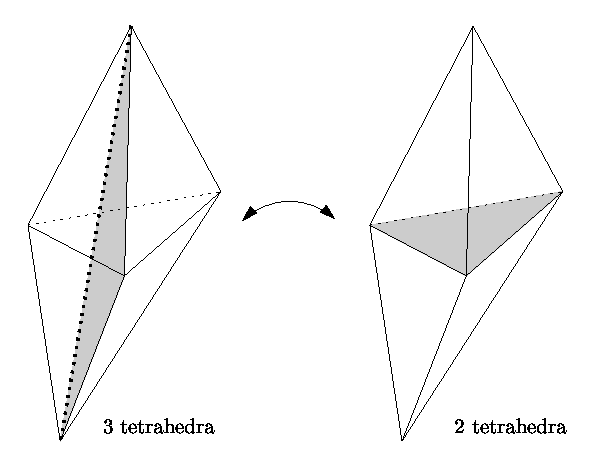
\includegraphics{flips.eps}
\end{center}
\end{ccTexOnly}
\caption{Flips.
\label{Triangulation3-fig-flips}}
\begin{ccHtmlOnly}
<CENTER>
<img border=0 src="./flips.gif" align=center
alt="Flips">
</CENTER>
\end{ccHtmlOnly}
\end{figure} 

The following methods guarantee the validity of the resulting 3D
triangulation.

\textit{Flips for a 2d triangulation are not implemented yet}

\ccMethod{bool flip(Edge e);}
\ccGlue
\ccMethod{bool flip(Cell_handle c, int i, int j);}
{Before flipping, these methods check that edge \ccc{e=(c,i,j)} is
flippable (which is quite expensive). They return \ccc{false} or
\ccc{true} according to this test.}

\ccMethod{void flip_flippable(Edge e);}
\ccGlue
\ccMethod{void flip_flippable(Cell_handle c, int i, int j);}
{Should be preferred to the previous methods when the edge is
known to be flippable.
\ccPrecond{The edge is flippable.}}

\ccMethod{bool flip(Facet f);}
\ccGlue
\ccMethod{bool flip(Cell_handle c, int i);}
{Before flipping, these methods check that facet \ccc{f=(c,i)} is
flippable (which is quite expensive). They return \ccc{false} or
\ccc{true} according to this test.} 

\ccMethod{void flip_flippable(Facet f);}
\ccGlue
\ccMethod{void flip_flippable(Cell_handle c, int i);}
{Should be preferred to the previous methods when the facet is
known to be flippable.
\ccPrecond{The facet is flippable.}}

\ccHeading{Insertions}

The following operations are guaranteed to lead to a valid triangulation 
when they are applied on a valid triangulation.

\ccMethod{Vertex_handle insert(const Point & p );}
{Inserts point \ccc{p} in the triangulation and returns the corresponding
 vertex.\\
If point \ccc{p} coincides with an already existing vertex, this 
vertex is returned and the triangulation remains unchanged.\\
If point \ccc{p} lies in the convex hull of the points, it is added
naturally: if it lies inside a cell, the cell is split into four
cells, if it lies on a facet, the two incident cells are split into
three cells, if it lies on an edge, all the cells incident to this
edge are split into two cells.\\
If point \ccc{p} is strictly outside the convex hull but in the affine
hull, \ccc{p} is linked to all visible points on the convex hull to
form the new triangulation. See
Figure~\ref{Triangulation3-fig-insert_outside_convex_hull}.\\  
If point \ccc{p} is outside the affine hull of the points, \ccc{p} is
linked to all the points, and the dimension of the triangulation is
incremented. All the points now belong to the boundary of the convex
hull, so, the infinite vertex is linked to all the points to
triangulate the new infinite face. See 
Figure~\ref{Triangulation3-fig-insert_outside_affine_hull}.}

\ccMethod{Vertex_handle insert(const Point & p, Cell_handle start);}
{Same as the previous method, but \ccc{start} is used as a starting
place for the search done within the insertion.}

\ccMethod{template < class InputIterator >
          int
          insert(InputIterator first, InputIterator last);}
{Inserts the points in the range $\left[\right.$\ccc{first},
\ccc{last}$\left.\right)$.  Returns the number of inserted points.
\ccPrecond{The \ccc{value_type} of \ccc{first} and \ccc{last} is
\ccc{Point}.}}
%\ccGlue
%\ccMethod{int insert(list<Point>::const_iterator first,
%	     list<Point>::const_iterator last);}
%{Same as the previous one.}
%\ccGlue
%\ccMethod{int insert(vector<Point>::const_iterator first,
%	     vector<Point>::const_iterator last);}
%{Same as the previous one.}
%\ccGlue
%\ccMethod{int insert(istream_iterator<Point, ptrdiff_t> first,
%	     istream_iterator<Point, ptrdiff_t> last);}
%{Same as the previous one.}
%\ccGlue
%\ccMethod{int insert(Point* first,
%	     Point* last);}
%{Same as the previous one.}

The previous methods are sufficient to build a whole triangulation. We
also provide some other methods that can be used instead of
\ccc{insert(p)} when the place where the new point \ccc{p} must be inserted
is already known. They are also guaranteed to lead to a valid
triangulation when they are applied on a valid triangulation.

\ccMethod{Vertex_handle insert_in_cell(const Point & p, Cell_handle c);} 
{Inserts point \ccc{p} in cell \ccc{c}. Cell \ccc{c} is split into 4
tetrahedra.
\ccPrecond{\ccVar.\ccc{dimension()} $=3$ and \ccc{p} lies strictly
inside cell \ccc{c}.}} 

\ccMethod{Vertex_handle insert_in_facet(const Point & p, const Facet & f);} 
{Inserts point \ccc{p} in facet \ccc{f}. In dimension~3, the 2
neighboring cells are split into 3 tetrahedra; in dimension~2, the facet 
is split into 3 triangles.
\ccPrecond{\ccVar.\ccc{dimension()} $\geq 2$ and \ccc{p} lies strictly
inside face \ccc{f}.}}
\ccGlue
\ccMethod{Vertex_handle insert_in_facet(const Point & p, 
					Cell_handle c, int i);}
{As above, insertion in facet \ccc{(c,i)}.
\ccPrecond{As above and $i \in \{0,1,2,3\}$ in dimension~3, $i = 3$ in
dimension~2.}}

\ccMethod{Vertex_handle insert_in_edge(const Point & p, const Edge & e);}
{Inserts \ccc{p} in edge \ccc{e}. In dimension~3, 
all the cells having this edge are split into 2 tetrahedra; in
dimension~2, the 2 neighboring facets are split into 2 triangles; in
dimension~1, the edge is split into 2 edges.
\ccPrecond{\ccVar.\ccc{dimension()} $\geq 1$ and \ccc{p} lies on edge
\ccc{e}.}}
\ccGlue
\ccMethod{Vertex_handle insert_in_edge(Point p, Cell_handle c, int i, int j);} 
{As above, inserts \ccc{p} in edge $(\ccc{i}, \ccc{j})$ of \ccc{c}.
\ccPrecond{As above and $i\neq j$. Moreover $i,j \in \{0,1,2,3\}$ in
dimension~3, $i,j \in \{0,1,2\}$ in dimension~2, $i,j \in \{0,1\}$ in 
dimension~1.}} 

\ccMethod{Vertex_handle insert_outside_convex_hull(const Point & p,
					Cell_handle c);}
%					int li, int lj=0);}
{%The cell \ccc{c}, together with \ccc{li} and possibly \ccc{lj}, give a
%separator (facet, edge or vertex, depending on the dimension) for
%\ccc{p} from the triangulation (see the description of method
%\ccc{locate()} for more details on the way the separator is represented).\\
The cell \ccc{c} must be an infinite cell containing \ccc{p}.\\
Links \ccc{p} to all  points in the triangulation that are visible from
\ccc{p}. Updates consequently the infinite faces. See
Figure~\ref{Triangulation3-fig-insert_outside_convex_hull}.
\ccPrecond{\ccVar.\ccc{dimension()} $>0$, \ccc{c}, and the $k$-face
represented by \ccc{c} is infinite and contains \ccVar.}}

\begin{figure}[htbp]
\begin{ccTexOnly}
\begin{center} 
\includegraphics{insert_outside_convex_hull.eps} 
\end{center}
\end{ccTexOnly}
\caption{\protect\ccc{insert_outside_convex_hull} (2-dimensional case).
\label{Triangulation3-fig-insert_outside_convex_hull}}
\begin{ccHtmlOnly}
<CENTER>
<img border=0 src="./insert_outside_convex_hull.gif" align=center alt="insert_outside_convex_hull} (2-dimensional case)">
</CENTER>
\end{ccHtmlOnly}
\end{figure} 

\ccMethod{Vertex_handle insert_outside_affine_hull(const Point & p);}
{\ccc{p} is linked to all the points, and the infinite vertex is linked
to all the points (including \ccc{p}) to triangulate the new infinite
face, so that all the points now belong to the boundary of the convex
hull. See Figure~\ref{Triangulation3-fig-insert_outside_affine_hull}.\\
This method can be used to insert the first point in an empty
triangulation.
\ccPrecond{\ccVar.\ccc{dimension()} $<3$ and \ccc{p} lies outside the
affine hull of the points.}} 

\begin{figure}[htbp]
\begin{ccTexOnly}
\begin{center} 
\includegraphics{insert_outside_affine_hull.eps} 
\end{center}
\end{ccTexOnly}
\caption{\protect\ccc{insert_outside_affine_hull} (2-dimensional case).
\label{Triangulation3-fig-insert_outside_affine_hull}}
\begin{ccHtmlOnly}
<CENTER>
<img border=0 src="./insert_outside_affine_hull.gif" align=center
alt="insert_outside_affine_hull} (2-dimensional case)">
</CENTER>
\end{ccHtmlOnly}
\end{figure} 

\ccHeading{Removal}

\ccMethod{void clear();}
{Removes all finite vertices and all cells of \ccVar.}

\ccHeading{Traversal of the Triangulation}

The triangulation class provides several iterators and circulators
that allow one to traverse it (completely or partially).

\ccHeading{Face, Edge and Vertex Iterators}
\ccThree{Facet_circulator}{t.finite_facets_begin()toto}{}

The following iterators allow the user to visit cells,
facets, edges and vertices of the
triangulation. These iterators are non-mutable, bidirectional and
their value types are respectively \ccc{Cell}, \ccc{Facet}, \ccc{Edge}
and \ccc{Vertex}. They are all invalidated by any change in the
triangulation. 

\ccMethod{Vertex_iterator finite_vertices_begin() const;}
{Starts at an arbitrary finite vertex. Then \ccc{++} and \ccc{--} will
iterate over finite vertices. Returns \ccc{vertices_end()} when
\ccVar.\ccc{number_of_vertices()} $<1$.} 
\ccGlue
\ccMethod{Vertex_iterator all_vertices_begin() const;}
{Starts at an arbitrary vertex. Iterates over all vertices (even infinite
ones). Returns \ccc{vertices_end()} when
\ccVar.\ccc{number_of_vertices()} $<1$.}  
\ccGlue
\ccMethod{Vertex_iterator vertices_end() const;}
{Past-the-end iterator}

\ccMethod{Edge_iterator finite_edges_begin() const;}
{Starts at an arbitrary finite edge. Then \ccc{++} and \ccc{--} will
iterate over finite edges. Returns \ccc{edges_end()} when
\ccVar.\ccc{dimension()} $<1$.} 
\ccGlue
\ccMethod{Edge_iterator all_edges_begin() const;}
{Starts at an arbitrary edge. Iterates over all edges (even infinite
ones). Returns \ccc{edges_end()} when \ccVar.\ccc{dimension()} $<1$.}
\ccGlue
\ccMethod{Edge_iterator edges_end() const;}
{Past-the-end iterator}

\ccMethod{Facet_iterator finite_facets_begin() const;}
{Starts at an arbitrary finite facet. Then \ccc{++} and \ccc{--} will
iterate over finite facets. Returns \ccc{facets_end()} when
\ccVar.\ccc{dimension()} $<2$.}
\ccGlue
\ccMethod{Facet_iterator all_facets_begin() const;}
{Starts at an arbitrary facet. Iterates over all facets (even infinite
ones). Returns \ccc{facets_end()} when 
\ccVar.\ccc{dimension()} $<2$.}
\ccGlue
\ccMethod{Facet_iterator facets_end() const;}
{Past-the-end iterator}

\ccMethod{Cell_iterator finite_cells_begin() const;}
{Starts at an arbitrary finite cell. Then \ccc{++} and \ccc{--} will
iterate over finite cells. Returns \ccc{cells_end()} when
\ccVar.\ccc{dimension()} $<3$.}
\ccGlue
\ccMethod{Cell_iterator all_cells_begin() const;}
{Starts at an arbitrary cell. Iterates over all cells (even infinite
ones). Returns \ccc{cells_end()} when 
\ccVar.\ccc{dimension()} $<3$.}
\ccGlue
\ccMethod{Cell_iterator cells_end() const;}
{Past-the-end iterator}

\ccHeading{Cell and facet circulators}

The following circulators respectively visit all cells or all facets
incident to a given edge. They are non-mutable and bidirectional. They
are invalidated by any modification of one of the cells traversed. 

\ccMethod{Cell_circulator incident_cells(Edge e) const;}
{Starts at an arbitrary cell incident to \ccc{e}.
\ccPrecond{\ccVar.\ccc{dimension()} $=3$.}}
\ccGlue
\ccMethod{Cell_circulator incident_cells(Cell_handle c, int i, int j) const;}
{As above for edge \ccc{(i,j)} of \ccc{c}.}
\ccGlue
\ccMethod{Cell_circulator incident_cells(Edge e, Cell_handle start) const;}
{Starts at cell \ccc{start}.
\ccPrecond{\ccVar.\ccc{dimension()} $=3$ and \ccc{start} is incident to
\ccc{e}.}}
\ccGlue
\ccMethod{Cell_circulator incident_cells(Cell_handle c, int i, int j, 
Cell_handle start) const;}
{As above for edge \ccc{(i,j)} of \ccc{c}.}

The following circulators on facets are defined only in dimension~3,
though facets are defined also in dimension~2: there are only two
facets sharing an edge in dimension~2. 
\ccMethod{Facet_circulator incident_facets(Edge e) const;}
{Starts at an arbitrary facet incident to \ccc{e}.
\ccPrecond{\ccVar.\ccc{dimension()}~$=3$}}
\ccGlue
\ccMethod{Facet_circulator incident_facets(Cell_handle c, int i, int j) const;}
{As above for edge \ccc{(i,j)} of \ccc{c}.} 
\ccGlue
\ccMethod{Facet_circulator incident_facets(Edge e, Facet start) const;}
{Starts at facet \ccc{start}. 
\ccPrecond{\ccc{start} is incident to \ccc{e}.}}
\ccGlue
\ccMethod{Facet_circulator incident_facets(Edge e, Cell_handle start, int f) 
const;}
{Starts at facet of index \ccc{f} in \ccc{start}.}
\ccGlue
\ccMethod{Facet_circulator incident_facets(Cell_handle c, int i, int j,
Facet start) const;} 
{As above for edge \ccc{(i,j)} of \ccc{c}.} 
\ccGlue
\ccMethod{Facet_circulator incident_facets(Cell_handle c, int i, int j,
Cell_handle start, int f) const;}
{As above for edge \ccc{(i,j)} of \ccc{c} and facet \ccc{(start,f)}.} 

\ccHeading{Traversal of the incident cells and the adjacent vertices
of a given vertex} 

\ccMethod{void incident_cells(Vertex_handle v, 
		set<Cell*, less<Cell*> > & cells,
		   Cell_handle c = NULL ) const;}
{Computes the set \ccc{cells} of all cells incident to \ccc{v}. If
\ccVar.\ccc{dimension()} $<3$ then the returned set is empty. The optional
argument \ccc{c} will be used for initializing the set.\\
\textit{This method computes a set of \ccc{Cell*}, whereas it should
logically compute a set of \ccc{Cell_handle}. This is due to
compilation problems with sets of \ccc{Cell_handle}. However, the user
can recover a \ccc{Cell_handle} for each element of the set by using
the method \ccc{handle()} defined for the \ccc{Cell} type.}
\ccPrecond{\ccc{v} $\neq$ \ccc{NULL}, \ccc{v} is a vertex of \ccVar\ 
and the optional argument \ccc{c} is a cell having \ccc{v} as vertex.}}

\ccMethod{void incident_vertices(Vertex_handle v, 
		set<Vertex*, less<Vertex*> > & vertices,
		Cell_handle c = NULL ) const;}
{Computes the set \ccc{vertices} of all vertices adjacent to \ccc{v}. If
\ccVar.\ccc{number_of_vertices()} $<1$ then the set is empty. The optional
argument \ccc{c} will be used for finding a first vertex of the set.\\
\textit{An analogous remark as for the previous method holds on the
types within the set.}
\ccPrecond{\ccc{v} $\neq$ \ccc{NULL}, \ccc{v} is a vertex of \ccVar\ and
the optional argument \ccc{c} is a cell having \ccc{v} as vertex.}}

\begin{ccAdvanced}
\ccHeading{Checking}
The responsibility of keeping a valid triangulation belongs to the user
when using advanced operations allowing a direct manipulation of cells
and vertices. We provide the user with the following methods to help
debugging. 

\ccMethod{bool
          is_valid(bool verbose = false) const;}
{Checks the combinatorial validity of the triangulation. Checks also the
validity of its geometric embedding (see
Section~\ref{Triangulation3-sec-Valid}).\\ When \ccc{verbose} is set to true, 
messages describing the first invalidity encountered are printed.}

\ccMethod{bool
          is_valid(Cell_handle c, bool verbose = false) const;}
{Checks the combinatorial validity of the cell by calling the
\ccc{is_valid} method of the \ccc{Tds} cell class. Also checks the
geometric validity of \ccc{c}, if \ccc{c} is finite. (See
Section~\pageref{Triangulation3-sec-Valid}.)\\ 
When \ccc{verbose} is set to \ccc{true}, messages are printed to give
a precise indication of the kind of invalidity encountered.}

These methods are mainly a debugging help for the users of advanced features.

\end{ccAdvanced}

\ccHeading{I/O}

\ccFunction{istream& operator>>
(istream& is, Triangulation_3<Traits, Tds> &t);}
{Reads the underlying combinatorial triangulation from \ccc{is} by
calling the corresponding input operator of the triangulation data
structure class, and the non-combinatorial information by calling the
corresponding input operators of the vertex and the cell
classes. Assigns the resulting triangulation to \ccc{t}.}

\ccFunction{ostream& operator<<
(ostream& os, const Triangulation_3<Traits, Tds> &t);}
{Writes the triangulation \ccc{t} into \ccc{os}.}

The information in the \ccc{iostream} is: the dimension, the number of
finite vertices, the non-combinatorial information about vertices (point,
etc), the number of cells, the indices of the vertices of each cell,
plus the non-combinatorial information about each cell, 
then the indices of the neighbors of each cell, where the index
corresponds to the preceding list of cells. When dimension $<$ 3, the
same information is stored for faces of maximal dimension instead of
cells. 

\end{ccClassTemplate}

\section{The Vertex of a Triangulation} 
\label{Triangulation3-sec-class-Vertex}

\begin{ccClassTemplate}{Triangulation_vertex_3<Traits,Tds>}
\ccCreationVariable{v}

\ccDefinition
The vertex stores a point and gives access to an incident face of
maximal dimension.

\ccInclude{CGAL/Triangulation_vertex_3.h}

\ccInheritsFrom{Tds::Vertex}

\ccTypes
\ccThree{typedef triple <Cell*, int, int>}{Facettoto}{}
The class \ccClassTemplateName\ defines the following types, also
defined in the class \ccc{Triangulation_3<Traits,Tds>}:

\ccTypedef{typedef Traits::Point Point;}{point type}
\ccGlue
\ccNestedType{Vertex_handle}{handle to a vertex}
\ccGlue
\ccNestedType{Cell_handle}{handle to a cell}

\begin{ccAdvanced}
\ccCreation
The user needs to construct vertices explicitly only when implementing his
own triangulation algorithms. If he uses the standard ways proposed by 
\cgal\ to construct a triangulation, he does not need the following
constructors. 

\ccConstructor{{Triangulation_vertex_3<Traits,Tds>}();}
{Introduces a new vertex. The geometric information is initialized by
the default constructor of the class \ccc{Point}. A test on the handle
to the incident cell of \ccVar\ for equality with \ccc{NULL} will
answer \ccc{true}.} 

\ccConstructor{{Triangulation_vertex_3<Traits,Tds>}(const Point & p);}
{Introduces vertex \ccVar, and initializes its geometric information.
A test on the handle
to the incident cell of \ccVar\ for equality with \ccc{NULL} will
answer \ccc{true}.}

\ccConstructor{{Triangulation_vertex_3<Traits,Tds>}(const Point & p,
                      		Cell_handle c);}
{Introduces vertex \ccVar, and initializes the geometric information and 
the handle to the incident cell.}

\ccConstructor{{Triangulation_vertex_3<Traits,Tds>}(Cell_handle c);}
{Introduces vertex \ccVar, and initializes the handle to the incident cell.}

\ccHeading{Setting}
\ccMethod{void set_cell(Cell_handle c);}
{Sets \ccVar's cell to \ccc{c}}
\ccMethod{void set_point(const Point & p);}
{Sets \ccVar's point to \ccc{p}}

\end{ccAdvanced}

\ccAccessFunctions

\ccMethod{Point point() const;}
{Returns the geometric information of \ccVar.}

\ccMethod{Cell_handle cell() const;}
{Finds a cell of the triangulation having \ccVar\ as
vertex. Remember that in degenerate dimensions, a cell stores a face
of maximal dimension (Section~\ref{Triangulation3-sec-degen_dim}).}

\ccMethod{Vertex_handle handle() const;}
{Returns a handle to the vertex.}

%\begin{ccAdvanced}
%\ccHeading{Checking}

%\ccMethod{bool is_valid(bool verbose = false) const;} 
%{Calls the \ccc{is_valid()} method of the \ccc{Tds} vertex class.\\
%When \ccc{verbose} is set to \ccc{true}, messages are printed to give
%a precise indication on the kind of invalidity encountered.} 
%\end{ccAdvanced} 

	\end{ccClassTemplate} 

\section{The Cell of a Triangulation} 
\label{Triangulation3-sec-class-Cell}

\begin{ccClassTemplate}{Triangulation_cell_3<Traits,Tds>}
\ccCreationVariable{c}

\ccDefinition

A cell of a triangulation gives access to its four vertices indexed 0,
1, 2, and 3 in positive orientation and to its four adjacent cells, also
called neighbors. The neighbors are indexed in such a way that neighbor
$i$ lies opposite to vertex $i$.

In degenerate dimensions, cells are used to store faces of maximal
dimension: (Section~\ref{Triangulation3-sec-degen_dim}).

\ccInclude{CGAL/Triangulation_cell_3.h}

\ccInheritsFrom{Tds::Cell}

\ccTypes
The class \ccClassTemplateName\ defines the same types as the
\ccc{Triangulation_vertex_3<Traits,Tds>} class.

\begin{ccAdvanced}
\ccCreation
The user needs to construct cells explicitly only when implementing his
own triangulation algorithms. The constructors of a cell do not insert
it into any triangulation. To add a cell to a given triangulation,
the \ccc{add_cell()} method of the triangulation must be used. Note
that a given cell can be inserted into only textit{one} triangulation.

\ccConstructor{Triangulation_cell_3<Traits,Tds>();}
{Introduces a cell \ccVar\ and initializes all its vertices and
neighbors in such a way that tests on the handles for equality with
\ccc{NULL} will answer \ccc{true}.} 

%\ccConstructor{\ccClassName(Tds & tds);}
%{Introduces a variable \ccVar, initializes the triangulation data
%structure related, and initializes all its vertices and
%neighbors as the preceding constructor.}

\ccConstructor{Triangulation_cell_3<Traits,Tds>(Vertex_handle v0,	
    	                    Vertex_handle v1,
                            Vertex_handle v2,
                            Vertex_handle v3);}
{Introduces a cell \ccVar, and initializes its vertices. The 
neighbors are initialized so that tests on the handles for equality with
\ccc{NULL} will answer \ccc{true}.} 

\ccConstructor{Triangulation_cell_3<Traits,Tds>(Vertex_handle v0,
                    	Vertex_handle v1,
                    	Vertex_handle v2,
                    	Vertex_handle v3,
                    	Cell_handle n0,
                    	Cell_handle n1,
                    	Cell_handle n2,
                    	Cell_handle n3);}
{Introduces a variable \ccVar, and initializes its vertices and neighbors.}

\ccHeading{Setting}
\ccThree{Cell_handle}{tds.set_number_of_vertices()}{}

\ccMethod{void set_vertices();}
{Sets all vertices so that tests on the handles for equality with
\ccc{NULL} will answer \ccc{true}.}
\ccGlue
\ccMethod{void set_vertex(int i, Vertex_handle v);}
{Sets vertex \ccc{i} of \ccVar\ to be \ccc{v}.
\ccPrecond{$i \in \{0,1,2,3\}$}}
\ccGlue
\ccMethod{void set_vertices(
	          Vertex_handle v0, 
                  Vertex_handle v1, 
                  Vertex_handle v2, 
                  Vertex_handle v3);}
{Sets vertices to the given vertices.}

\ccMethod{void set_neighbors();}
{Sets all neighbors so that tests on the handles for equality with
\ccc{NULL} will answer \ccc{true}.}
\ccGlue
\ccMethod{void set_neighbor(int i, Cell_handle n);}
{Sets neighbor \ccc{i} to be \ccc{n}.
\ccPrecond{$i \in \{0,1,2,3\}$.}}
\ccGlue
\ccMethod{void set_neighbors(
                  Cell_handle n0,
                  Cell_handle n1,  
                  Cell_handle n2,  
                  Cell_handle n3);}
{Sets neighbors to the given cells.}
\end{ccAdvanced} 

\ccAccessFunctions
\ccThree{Vertex_handle}{c.has_vertex( Vertex_handle) v)}{}

\ccMethod{Vertex_handle vertex(int i) const;}
{Returns vertex \ccc{i} of \ccVar.
\ccPrecond{$i \in \{0,1,2,3\}$.}}
\ccGlue
\ccMethod{int index(Vertex_handle v) const;}
{Returns the index of vertex \ccc{v} in \ccVar.
\ccPrecond{\ccc{v} is a vertex of \ccVar.}}
\ccGlue
\ccMethod{bool has_vertex(Vertex_handle v) const;}
{Returns \ccc{true} if  \ccc{v} is a vertex of \ccVar.}
\ccGlue
\ccMethod{bool has_vertex(Vertex_handle v, int & i) const;}
{Returns \ccc{true} if \ccc{v} is a vertex of \ccVar, and
computes the index \ccc{i} of the vertex.}

\ccMethod{Cell_handle neighbor(int i) const;}
{Returns neighbor \ccc{i} of \ccVar.
\ccPrecond{$i \in \{0,1,2,3\}$.}}
\ccGlue
\ccMethod{int index(Cell_handle n) const;}
{Returns the index corresponding to neighboring cell \ccc{n}.
\ccPrecond{\ccc{n} is a neighbor of \ccVar.}}
\ccGlue
\ccMethod{bool has_neighbor(Cell_handle n) const;}
{Returns \ccc{true} if \ccc{n} is a neighbor of \ccVar.}
\ccGlue
\ccMethod{bool has_neighbor(Cell_handle n, int & i) const;}
{Returns \ccc{true} if \ccc{n} is a neighbor of \ccVar, and
computes the index \ccc{i} of the neighbor.}

\ccMethod{Cell_handle handle() const;}
{Returns a handle to the cell.}

	\end{ccClassTemplate} 



\section{Delaunay Triangulation} 

\begin{ccClassTemplate}{Delaunay_triangulation_3<Traits,Tds>}
\ccDefinition
\ccInclude{CGAL/Delaunay_triangulation_3.h}

\ccInheritsFrom{\ccc{Triangulation_3<Traits,Tds>}}

\ccCreationVariable{dt}

\ccTypes

Inherits the types of \ccc{Triangulation_3<Traits,Tds>}.

\ccCreation
\ccThree{Vertex_handle}{dt.remove(Pont p)toto}{}

\ccConstructor{Delaunay_triangulation_3<Traits,Tds>()}
{Creates an empty Delaunay triangulation.}

\ccConstructor{Delaunay_triangulation_3<Traits,Tds>(const Traits & traits)}
{Creates an empty Delaunay triangulation with traits class
\ccc{traits}.}

\ccConstructor{Delaunay_triangulation_3<Traits,Tds>(const Delaunay_triangulation_3<Traits,Tds> & dt1)}
{Copy constructor.}

\ccModifiers

\ccHeading{Insertion}

The following methods overload the corresponding methods of
triangulations to ensure the empty sphere property of Delaunay 
triangulations.

\ccMethod{Vertex_handle insert(const Point & p );}
{Inserts point \ccc{p} in the triangulation and returns the corresponding
 vertex. Similar to the insertion in a triangulation, but ensures in
addition the empty sphere property of all the created faces.}

\ccMethod{Vertex_handle insert(const Point & p, Cell_handle start);}
{Same as the previous method, \ccc{start} is used as a starting
place for the search done within the insertion.}

The following method allows one to insert several points. It returns the
number of inserted points. 

\ccMethod{template < class InputIterator >
          int
          insert(InputIterator first, InputIterator last);}
{Inserts the points in the range $\left[\right.$\ccc{first},
\ccc{last}$\left.\right)$. 
\ccPrecond{The \ccc{value_type} of \ccc{first} and \ccc{last} is
\ccc{Point}.}}
%\ccMethod{int insert(list<Point>::const_iterator first,
%	     list<Point>::const_iterator last);}
%{}
%\ccGlue
%\ccMethod{int insert(vector<Point>::const_iterator first,
%	     vector<Point>::const_iterator last);}
%{}
%\ccGlue
%\ccMethod{int insert(istream_iterator<Point, ptrdiff_t> first,
%	     istream_iterator<Point, ptrdiff_t> last);}
%{}
%\ccGlue
%\ccMethod{int insert(Point* first,
%	     Point* last);}
%{}

\ccHeading{Removal}

\ccMethod{void remove(Point p);}
{Removes the vertex associated with \ccc{p}.
\ccPrecond{There is a vertex of the triangulation associated with \ccc{p}.}\\
\textit{not yet implemented}}

\ccHeading{Queries}

\ccMethod{Bounded_side
          side_of_sphere(Cell_handle c, const Point & p) const;}
{Returns a value indicating on which side of the circumscribed sphere
of \ccc{c} the point \ccc{p} lies. More precisely, it returns:\\
- \ccc{ON_BOUNDED_SIDE} if \ccc{p} is inside the sphere. For an infinite
cell this means that \ccc{p} lies strictly either in the half space
limited by its finite facet and not containing any other point of the
triangulation, or in the interior of the disk circumscribing the
\textit{finite} facet. \\ 
- \ccc{ON_BOUNDARY} if p on the boundary of the sphere. For an infinite
cell this means that \ccc{p} lies on the circle circumscribing
the \textit{finite} facet.\\ 
- \ccc{ON_UNBOUNDED_SIDE} if \ccc{p} lies outside the sphere. For an
infinite cell this means that \ccc{p} does not satisfy either of the
two previous conditions. 
\ccPrecond{\ccVar.\ccc{dimension()} $=3$.}}
\ccMethod{Bounded_side
	  side_of_circle(const Facet & f, const Point & p) const;}
{Returns a value indicating on which side of the circumscribed circle
of \ccc{f} the point \ccc{p} lies. More precisely, it returns:\\
- in dimension~3:\\
-- For a finite facet, \ccc{ON_BOUNDARY} if \ccc{p} lies
on the circle, \ccc{ON_UNBOUNDED_SIDE} when it lies in the exterior of
the disk, \ccc{ON_BOUNDED_SIDE} when it lies in its interior.\\
-- For an infinite facet, it considers the plane defined by the finite
facet of the same cell, and does the same as in dimension~2 in this
plane.\\
- in dimension~2:\\
-- For a finite facet, \ccc{ON_BOUNDARY} if \ccc{p} lies
on the circle, \ccc{ON_UNBOUNDED_SIDE} when it lies in the exterior of
the disk, \ccc{ON_BOUNDED_SIDE} when it lies in its interior.\\
-- For an infinite facet, \ccc{ON_BOUNDARY} if the
point lies on the finite edge of \ccc{f} (endpoints included),
\ccc{ON_BOUNDED_SIDE} for a point in the open half plane defined
by \ccc{f} and not containing any other point of the triangulation,
\ccc{ON_UNBOUNDED_SIDE} elsewhere. 
\ccPrecond{\ccVar.\ccc{dimension()} $\geq 2$ and in dimension 3,
\ccc{p} is coplanar with \ccc{f}.}}

\ccMethod{Bounded_side
	  side_of_circle(Cell_handle c, int i, const Point & p);}
{Same as the previous method for facet \ccc{i} of cell \ccc{c}.}

\begin{ccAdvanced}
\ccHeading{Checking}
\ccMethod{bool
          is_valid(bool verbose = false) const;}
{Checks the combinatorial validity of the triangulation and the
validity of its geometric embedding (see
Section~\ref{Triangulation3-sec-Valid}). Also checks that all the
circumscribing spheres (resp. circles in dimension~2) of  cells
(resp. facets in dimension~2) are empty.\\ When \ccc{verbose} is set to
true,  messages describing the first invalidity encountered are
printed.}

\ccMethod{bool
          is_valid(Cell_handle c, bool verbose = false) const;}
{Checks the combinatorial and geometric validity of the cell (see
Section~\ref{Triangulation3-sec-Valid}). Also checks that the
circumscribing sphere (resp. circle in dimension~2) of  cells
(resp. facet in dimension~2) is empty.\\
 When \ccc{verbose} is set to
true, messages are printed to give
a precise indication of the kind of invalidity encountered.}

These methods are  mainly a debugging help for the users of advanced features.
\end{ccAdvanced}

\end{ccClassTemplate}

\section{Hierarchic Delaunay Triangulation} 

(See~\cite{d-iirdt-98}.)

\begin{ccClassTemplate}{Delaunay_hierarchic_triangulation_3<Traits,Tds>}

\textit{Not yet implemented}

\end{ccClassTemplate}

\section{Regular Triangulation} 
\label{Triangulation3-sec-class-Regulartriangulation}

\begin{ccClassTemplate}{Regular_triangulation_3<Traits,Tds>}
\ccDefinition

Let ${S}^{(w)}$ be a set of weighted points in $\R^3$. Let
${p}^{(w)}=(p,w_p), p\in\R^3, w_p\in\R$ and 
${z}^{(w)}=(z,w_z), z\in\R^3, w_z\in\R$ be two weighted points. 
A weighted point
${p}^{(w)}=(p,w_p)$ can also be seen as a sphere of center $p$ and
radius $w_p$. 
The \textit{power product} between ${p}^{(w)}$ and ${z}^{(w)}$ is
defined as 
\[\Pi({p}^{(w)},{z}^{(w)}) = {\|{p-z}\|^2-w_p^2-w_z^2}\]
where $\|{p-z}\|$ is the Euclidean distance between $p$ and $z$. 
 ${p}^{(w)}$ and ${z}^{(w)}$
are said to be \textit{orthogonal} if $\Pi{({p}^{(w)}-{z}^{(w)})}
= 0$ (see Figure~\ref{Triangulation3-fig-ortho}).

\begin{figure}[htbp]
\begin{ccTexOnly}
\begin{center} 
\includegraphics{ortho.eps} 
\end{center}
\end{ccTexOnly}
\caption{Orthogonal weighted points (picture in 2D).
\label{Triangulation3-fig-ortho}}
\begin{ccHtmlOnly}
<CENTER>
<img border=0 src="./ortho.gif" align=center alt="Orthogonal weighted
points (picture in 2D)"> 
</CENTER>
\end{ccHtmlOnly}
\end{figure} 

Four weighted points have a unique common orthogonal weighted point called
the \textit{power sphere}. A sphere ${z}^{(w)}$ is said to be
\textit{regular} if $\forall {p}^{(w)}\in{S}^{(w)},
\Pi{({p}^{(w)}-{z}^{(w)})}\geq 0$.

A triangulation of ${S}^{(w)}$ is \textit{regular} if the power spheres
of all simplices are regular. 

The regular triangulation of
${S}^{(w)}$ is in fact the projection onto $\R^3$ of the convex hull 
of the four-dimensional points $(p,\|p-O\|^2-w_p),$ for
${p}^{(w)}=(p,w_p)\in{S}^{(w)}$. 
Note that all points of ${S}^{(w)}$ do not
necessarily appear as vertices of the regular
triangulation. To know more about regular triangulations, see for
example \cite{es-itfwr-96}. 

When all weights are 0, power spheres are nothing more than
circumscribing spheres, and the regular triangulation is exactly the
Delaunay triangulation.

We will call the weighted point orthogonal to three weighted points in
the plane defined by these three points the \textit{power circle}. The
\textit{power segment} will denote the weighted point orthogonal to
two weighted points on the line defined by these two points.

To simplify notation, $p$ will often denote in the sequel either the
point $p\in\R^3$ or the weighted point ${p}^{(w)}=(p,w_p)$.

\ccInclude{CGAL/Regular_triangulation_3.h}

\ccInheritsFrom{\ccc{Triangulation_3<Traits,Tds>}}

\ccCreationVariable{rt}

\ccTypes
\ccThree{typedef Traits::Weighted_point}{Weighted_point}{}

Inherits the types of \ccc{Triangulation_3<Traits,Tds>}.

\ccTypedef{typedef Traits::Bare_point Bare_point;}{The type for points
\ccc{p} of weighted points ${p}^{(w)}=(p,w_p)$}
\ccGlue
\ccTypedef{typedef Traits::Weighted_point Weighted_point;}{}

\ccCreation
\ccThree{Regular_triangulation_3<Traits,Tds>}{rt( Traits traits );xxx}{}

\ccConstructor{Regular_triangulation_3<Traits,Tds>()}
{Creates an empty regular triangulation.}

\ccConstructor{Regular_triangulation_3<Traits,Tds>(const Traits & traits)}
{Creates an empty regular triangulation with traits class
\ccc{traits}.}

\ccConstructor{Regular_triangulation_3<Traits,Tds>(const Regular_triangulation_3<Traits,Tds> & dt1)}
{Copy constructor.}

\ccModifiers

\ccHeading{Insertion}
\ccThree{Vertex_handle}{dt.insertxx}{}

The following methods, which already exist in triangulations, are
overloaded to ensure the property that all power spheres are regular.

\ccMethod{Vertex_handle insert(const Weighted_point & p );}
{Inserts weighted point \ccc{p} in the triangulation. If this
insertion creates a vertex, this vertex is returned. Otherwise, this
method returns \ccc{NULL}.}

\ccMethod{Vertex_handle insert(const Weighted_point & p, Cell_handle start);}
{Same as the previous method, \ccc{start} is used as a starting
place for the search done within the insertion.}

The following method allows one to insert several points. It returns the
number of inserted points. 

\ccMethod{template < class InputIterator >
          int
          insert(InputIterator first, InputIterator last);}
{Inserts the points in the range $\left[\right.$\ccc{first},
\ccc{last}$\left.\right)$. 
\ccPrecond{The \ccc{value_type} of \ccc{first} and \ccc{last} is
\ccc{Point}.}}

\ccHeading{Queries}
\ccThree{Bounded_side}{rt.side of powerxx}{}

Let us remark that 
\[\Pi({p}^{(w)}-{z}^{(w)}) > 0\]
is equivalent to\\
\centerline{\ccc{p} lies outside the sphere with center \ccc{z} and radius
$\sqrt{w_p^2+w_z^2}$.}\\
This remark helps provide an intuition about the following predicates.

\begin{figure}[htbp]
\begin{ccTexOnly}
\begin{center} 
\includegraphics{sidedim2.eps} 
\end{center}
\end{ccTexOnly}
\caption{side\_of\_power\_circle.
\label{Triangulation3-fig-sidedim2}}
\begin{ccHtmlOnly}
<CENTER>
<img border=0 src="./sidedim2.gif" align=center
alt="side\_of\_power\_circle"> 
</CENTER>
\end{ccHtmlOnly}
\end{figure} 

\ccMethod{Bounded_side
          side_of_power_sphere(Cell_handle c, const Weighted_point & p) const;}
{Returns the position of the weighted point $p$ with respect to the
power sphere of \ccc{c}. More precisely, it returns:\\
- \ccc{ON_BOUNDED_SIDE} if $\Pi({p}^{(w)}-{z(c)}^{(w)})<0$ where
${z(c)}^{(w)}$ is the power sphere of \ccc{c}. For an
infinite cell this means either that \ccc{p} lies strictly in the half
space limited by its finite facet and not containing any other point
of the triangulation, or that the angle 
between \ccc{p} and the power circle of the \textit{finite} facet of \ccc{c}
is greater than $\pi/2$. \\  
- \ccc{ON_BOUNDARY} if p is orthogonal to the power sphere of \ccc{c}
i.e. $\Pi({p}^{(w)}-{z(c)}^{(w)})=0$. For an infinite cell this means
that \ccc{p} is orthogonal to the power circle of its \textit{finite} facet.\\ 
- \ccc{ON_UNBOUNDED_SIDE} if $\Pi({p}^{(w)}-{z(c)}^{(w)})>0$
i.e. the angle between the weighted point \ccc{p} and the power sphere
of \ccc{c} is less than $\pi/2$ or if these two spheres do not
intersect. For an 
infinite cell this means that \ccc{p} does not satisfy either of the
two previous conditions. 
\ccPrecond{\ccVar.\ccc{dimension()} $=3$.}}

\ccMethod{Bounded_side
	  side_of_power_circle(const Facet & f, 
			const Weighted_point & p) const;}
{Returns the position of the point \ccc{p} with respect to the
power circle of \ccc{f}. More precisely, it returns:\\
--- in dimension~3:\\
-- For a finite facet,\\
\ccc{ON_BOUNDARY} if \ccc{p} is orthogonal to the power circle in the
plane of the facet,\\ 
\ccc{ON_UNBOUNDED_SIDE} when their angle is less than $\pi/2$,\\
\ccc{ON_BOUNDED_SIDE} when it is greater than $\pi/2$ (see
Figure~\ref{Triangulation3-fig-sidedim2}).\\ 
-- For an infinite facet, it considers the plane defined by the finite
facet of the cell \ccc{f.first}, and does the same as in
dimension~2 in this plane.\\
--- in dimension~2:\\
-- For a finite facet,\\
\ccc{ON_BOUNDARY} if \ccc{p} is orthogonal to the circle,\\
\ccc{ON_UNBOUNDED_SIDE} when the angle between \ccc{p} and the
power circle of \ccc{f} is less than $\pi/2$,
\ccc{ON_BOUNDED_SIDE} when it is greater than $\pi/2$.\\ 
-- For an infinite facet,\\
\ccc{ON_BOUNDED_SIDE} for a point in the open half plane defined by
\ccc{f} and not containing any other point of the triangulation,\\
\ccc{ON_UNBOUNDED_SIDE} in the other open half plane.\\
If the point \ccc{p} is collinear with the finite edge \ccc{e} of
\ccc{f}, it returns:\\
\ccc{ON_BOUNDED_SIDE} if $\Pi({p}^{(w)}-{z(e)}^{(w)})<0$, where
${z(e)}^{(w)}$ is the power segment of \ccc{e} in the line supporting
\ccc{e},\\ 
\ccc{ON_BOUNDARY} if $\Pi({p}^{(w)}-{z(e)}^{(w)})=0$,\\
\ccc{ON_UNBOUNDED_SIDE} if $\Pi({p}^{(w)}-{z(e)}^{(w)})>0$ .
\ccPrecond{\ccVar.\ccc{dimension()} $\geq 2$.}}

\ccMethod{Bounded_side
	  side_of_power_circle(Cell_handle c, int i, 
			const Weighted_point & p) const;}
{Same as the previous method for facet \ccc{i} of cell \ccc{c}.}

\ccMethod{Bounded_side
	  side_of_power_segment(Cell_handle c, const Weighted_point & p)
const;}
{In dimension~1, returns\\
\ccc{ON_BOUNDED_SIDE} if $\Pi({p}^{(w)}-{z(c)}^{(w)})<0$, where
${z(c)}^{(w)}$ is the power segment of the edge represented by
\ccc{c},\\
\ccc{ON_BOUNDARY} if $\Pi({p}^{(w)}-{z(c)}^{(w)})=0$,\\
\ccc{ON_UNBOUNDED_SIDE} if $\Pi({p}^{(w)}-{z(c)}^{(w)})>0$ .
\ccPrecond{\ccVar.\ccc{dimension()} $= 1$.}}

\begin{ccAdvanced}
\ccHeading{Checking}
\ccMethod{bool
          is_valid(bool verbose = false) const;}
{Checks the combinatorial validity of the triangulation and the
validity of its geometric embedding (see
Section~\ref{Triangulation3-sec-Valid}). Also checks that all the
power spheres (resp. power circles in dimension~2, power segments in
dimension~1) of cells (resp. facets in dimension~2, edges in
dimension~1) are regular. When \ccc{verbose}
is set to true, messages describing the first invalidity encountered
are printed.\\ This method is mainly a debugging help for the users of
advanced features.
}
\end{ccAdvanced}

\end{ccClassTemplate}

%\section{Debugging}

%	\subsection{Pretty print}	
% \textit{to be written}

%	\subsection{Debugging with handles} 
%Most debuggers cannot understand \ccc{handles} well. Under the
%debugger, an instruction such as

%\texttt{(dbx) print -r c->vertex(0)}

%where \ccc{c} is a \ccc{Cell_handle}, is answered by:

%\texttt{can't find field "vertex" in "c"}

%To work around this problem, two functions have been defined to transform 
%\ccc{handles} into usual $C^{++}$ pointers for debugging purposes.

%\ccFunction{template <class Traits, class Tds>
%	Triangulation_vertex_3<Traits,Tds> * 
%debug(const Triangulation_vertex_handle_3<Traits,Tds> v);}
%{}

%\ccFunction{template <class Traits, class Tds>
%	Triangulation_cell_3<Traits,Tds> * 
%	debug(const Triangulation_cell_handle_3<Traits,Tds>
%c);}
%{}

%This allows the following:\\
%\texttt{(dbx) print -r CGAL\_debug(c)->vertex(0)\\
%CGAL\_debug(c)->vertex(0) = \{\\\
%\ldots\\
%\} }

\section{The Geometric Traits}
\label{Triangulation3-sec-Traits}

The first template parameter of the triangulation class
\ccc{Triangulation_3<Traits,Tds>} of \cgal\ is the geometric traits class.

The first subsection of this section describes the requirements
that a geometric traits class must fulfill. The second subsection
presents a predefined geometric traits class available in \cgal.

	
	\subsection{Concept for the Geometric Traits Class}
	\label{Triangulation3-sec-concept-Traits}

	\begin{ccClass}{Triangulation_Traits_3}
\subsubsection{To be used by \protect \ccc{Triangulation_3<Traits, Tds>}}

\ccCreationVariable{traits}

The geometric traits class \ccClassName\ of the triangulation
class \ccc{Triangulation_3<Traits, Tds>} must define the geometric
objects (points, segments, triangles and tetrahedra) forming the
triangulation together with a few geometric predicates on these objects:
equality, coordinate comparison, orientation in space, orientation
in case of coplanar points, and collinearity tests.

\ccTypes
\ccThree{Traits::Tetrahedron}{tds.set_number_of_vertices()}{}

\ccNestedType{Point}
{The type must provide a copy constructor and assignment operator.}
\ccGlue
\ccNestedType{Segment}
{The  type must provide a constructor that takes two points as arguments.}
\ccGlue
\ccNestedType{Triangle}
{The type must provide a constructor that takes three points as
arguments.}
\ccGlue
\ccNestedType{Tetrahedron}
{The type must provide a constructor that takes four points as
arguments.}

\ccCreation
\ccThree{Comparison_result}{compare_x()toto}{}

Only a default constructor is required.

\ccConstructor{Traits();} 
{A default constructor.}
%\ccGlue
%\ccConstructor{\ccClassName(const Traits & traits1);}
%{Copy constructor.}
%\ccGlue
%\ccMethod{Traits operator=(const Traits & traits1);}
%{Assignment.}

\ccHeading{Predicates}
\ccMethod{bool equal(const Point & p, const Point & q) const;}
{Equality test.}

\ccMethod{Comparison_result compare_x(const Point & p, const Point
& q) const;}
{Comparison of \ccc{x}-coordinates. Returns \ccc{LARGER}
(resp. \ccc{EQUAL}, \ccc{SMALLER}) when the \ccc{x}
coordinate of \ccc{p} is larger than (resp. equal to, smaller than)
the \ccc{x} coordinate of \ccc{q}.} 
\ccGlue
\ccMethod{Comparison_result compare_y(const Point & p, const Point
& q) const;}
{Comparison of \ccc{y}-coordinates.}
\ccGlue
\ccMethod{Comparison_result compare_z(const Point & p, const Point
& q) const;}
{Comparison of \ccc{z}-coordinates.}

\ccMethod{Orientation orientation(const Point& p0,
                                       const Point& p1,
                                       const Point& p2,
                                       const Point& p3) const;}
{Orientation test in three dimensions.}

\ccMethod{Orientation orientation_in_plane
				(const Point & q,	
				 const Point & r,
				 const Point & s,
				 const Point & test) const;}
{Tests whether \ccc{test} is on the same side of \ccc{(q, r)} as
\ccc{s} in the common plane of the four points. Returns \ccc{COLLINEAR} if
\ccc{test, q, r} are collinear, \ccc{POSITIVE} if \ccc{(q, r, test)}
and \ccc{(q, r, s)} have the same orientation, \ccc{NEGATIVE} if
\ccc{(q, r, test)} and \ccc{(q, r, s)} have opposite orientations. 
\ccPrecond{\ccc{test, q, r, s} are coplanar and \ccc{q, r, s} are not
collinear.}} 

\ccMethod{bool collinear(const Point & p,
		 	 const Point & q,
		 	 const Point & r) const;}
{Collinearity test.}

\subsubsection{To be used by \protect 
\ccc{Delaunay_triangulation_3<Traits, Tds>}}

In addition to the requirements described before, the geometric traits
class of a 
Delaunay triangulation must fulfill the following requirements:

\ccHeading{Predicates}

\ccMethod{Oriented_side 
  	side_of_oriented_sphere(const Point & p,
			  const Point & q,
			  const Point & r,
			  const Point & s,
			  const Point & test) const;}
{Determines on which side of the oriented sphere circumscribing 
\ccc{p, q, r, s} the point \ccc{test} lies.} 

\ccMethod{Oriented_side 
  side_of_oriented_circle(const Point & p,
			  const Point & q,
			  const Point & r,
			  const Point & test) const;}
{Determines on which side of the oriented circle circumscribing
\ccc{p, q, r} the point \ccc{test} lies. 
\ccPrecond{\ccc{p, q, r, test} are coplanar and \ccc{p, q, r} are not
collinear.}}  

\subsubsection{To be used by \protect 
\ccc{Delaunay_hierarchic_triangulation_3<Traits, Tds>}}

\textit{Not yet implemented}

\subsubsection{To be used by \protect 
\ccc{Regular_triangulation_3<Traits, Tds>}}

To be used as the traits class for the regular triangulation provided
by \cgal, a class must satisfy additional requirements.

We use here the same notation as in
Section~\ref{Triangulation3-sec-class-Regulartriangulation}. 

\ccMethod{Oriented_side power_test(const Weighted_point &p,
			   const Weighted_point &q,
			   const Weighted_point &r,
			   const Weighted_point &s,
			   const Weighted_point &t) const;}
{Let ${z(p,q,r,s)}^{(w)}$ be the power sphere of the weighted points 
$(p,q,r,s)$. Returns \\
\ccc{ON_ORIENTED_BOUNDARY} if \ccc{t} is orthogonal to
${z(p,q,r,s)}^{(w)}$,\\ 
\ccc{ON_NEGATIVE_SIDE} if \ccc{t} lies outside the oriented sphere of
center $z(p,q,r,s)$ and radius $\sqrt{ w_{z(p,q,r,s)}^2 + w_t^2 }$
(which is equivalent to $\Pi({t}^{(w)},{z(p,q,r,s)}^{(w)} >0$)),\\
\ccc{ON_POSITIVE_SIDE} if \ccc{t} lies inside this oriented sphere.
\ccPrecond{\ccc{p, q, r, s} are not coplanar.}}

Note that with this definition, if all the points have a weight equal
to 0, then
\ccc{power_test(p,q,r,s,t)} = \ccc{side_of_oriented_sphere(p,q,r,s,t)}.

\ccMethod{Oriented_side power_test(const Weighted_point &p,
			   const Weighted_point &q,
			   const Weighted_point &r,
			   const Weighted_point &t) const;}
{Analogous definition as the previous method, for coplanar points,
with the power circle ${z(p,q,r)}^{(w)}$.
\ccPrecond{\ccc{p, q, r} are not collinear and \ccc{p, q, r, t} are
coplanar.}}

If all the points have a weight equal to 0, then
\ccc{power_test(p,q,r,s,t)} = \ccc{side_of_oriented_circle(p,q,r,s,t)}.

\ccMethod{Oriented_side power_test(const Weighted_point &p,
			   const Weighted_point &q,
			   const Weighted_point &t) const;}
{Same for collinear points, where ${z(p,q)}^{(w)}$ is the
power segment of \ccc{p} and \ccc{q}.
\ccPrecond{\ccc{p} and \ccc{q} have different Bare\_points, and
\ccc{p, q, t} are collinear.}}

If all the points have a weight equal to 0, then
\ccc{power_test(p,q,t)} gives the same answer as the kernel predicate
\ccc{s(p,q).has_on(t)} would give, where  \ccc{s(p,q)} denotes the
segment with endpoints \ccc{p} and \ccc{q}.

	\end{ccClass} 

	\subsection{Model for the traits class} 
	\label{Triangulation3-sec-class-Traits}

	\begin{ccClassTemplate}{Triangulation_geom_traits_3<R>}
\cgal\ provides a predefined geometric traits class using the kernel
geometric objects and predicates.
This class is templated with a representation class.

The traits class \ccClassTemplateName\ is designed to deal with \cgal\ three
dimensional points. It supplies the user with all
the functionalities described in
Section~\ref{Triangulation3-sec-concept-Traits}.
So, it can be used as a default traits
class for \ccc{Triangulation_3<Traits,Tds>},
\ccc{Delaunay_triangulation_3<Traits,Tds>} and
\ccc{Delaunay_hierarchic_triangulation_3<Traits,Tds>}.

\ccInclude{CGAL/Triangulation_geom_traits_3.h}

\ccTypes
\ccThree{typedef triple <Cell*, int, int>}{Facet }{}

\ccTypedef{typedef Point_3<R> Point;}{}
\ccGlue
\ccTypedef{typedef Segment_3<R> Segment;}{}
\ccGlue
\ccTypedef{typedef Triangle_3<R> Triangle;}{}
\ccGlue
\ccTypedef{typedef Tetrahedron_3<R> Tetrahedron;}{}

	\end{ccClassTemplate} 

	\subsection{Model for the traits class of a regular triangulation} 
	\label{Triangulation3-sec-class-Regulartraits}

	\begin{ccClassTemplate}{Regular_triangulation_euclidean_traits_3<R,Weight>}
This traits class is designed to be used by the class
\ccc{Regular_triangulation_3<Traits,Tds>}. It provides
\ccc{Weighted_point}, a class for weighted points
provided by the class, which derives from the \cgal\ three dimensional
point class (see
Section~\ref{Triangulation3-sec-class-Weightedpoints}). It supplies
the user with all the functionalities 
described in Section~\ref{Triangulation3-sec-concept-Traits}.
 It can be used as a default traits
class for \ccc{Regular_triangulation_3<Traits,Tds>}.

The second argument \ccc{Weight} of the class
\ccc{Regular_triangulation_euclidean_traits_3<R,Weight>} is in fact
optional: if is it not provided, \ccc{R::RT} will be used.

\ccInclude{CGAL/Regular_triangulation_euclidean_traits_3.h}

\ccInheritsFrom{\ccc{Triangulation_geom_traits_3<R>}}

\ccTypes
\ccThree{typedef Triangulation_geom_traits_3::Point}{Weighted_point;}{}

\ccTypedef{typedef Triangulation_geom_traits_3::Point Bare_point;}{The
type for point $p$ of a weighted point ${p}^{(w)}=(p,w_p)$.}
\ccGlue
\ccTypedef{typedef Weighted_point <Bare_point, Weight> Weighted_point;}{}

As \ccClassTemplateName\ inherits from
\ccc{Triangulation_geom_traits_3<R>}, the \ccc{Bare_point} type is in
fact \ccc{Point_3<R>}.

	\end{ccClassTemplate}

		\subsection{Weighted point}	
		\label{Triangulation3-sec-class-Weightedpoints}

		\subsubsection{Concept for a weighted point}

The weighted point class must fulfill the following requirements:

\ccTypes
\ccThree{typedef Point::RT}{RTxxxx}{}
\ccNestedType{Point Point}{The point type}
\ccGlue
\ccNestedType{Weight Weight}{The weight type}
\ccGlue
\ccTypedef{typedef Point::RT RT;}{The ring type}

\ccCreation
\ccCreationVariable{wp}

\ccConstructor{Weighted_point(const Point &p=Point(), const Weight &w
= Weight(0))}{}

\ccAccessFunctions
\ccFunction{Point point() const;}{}
\ccFunction{Weight weight() const;}{}

		\subsubsection{Model of weighted point} 

		\begin{ccClassTemplate}{Weighted_point<Point,Weight>}
This class provides \ccc{Regular_triangulation_euclidean_traits_3}
with all the required functionalities.

\ccInclude{CGAL/Weighted_point.h}

\ccInheritsFrom{\ccc{Point} (the template parameter) }

		\end{ccClassTemplate}

\section{The Triangulation Data Structure Parameter}
\label{Triangulation3-sec-tds}

The second template parameter of the basic triangulation class
\ccc{Triangulation_3<Traits,Tds>} is a triangulation data structure
class.  This class can be seen as a container for the cells and
vertices maintaining incidence and adjacency relations. 

The concept for the triangulation data structure is described in
Section~\ref{TDS3-sec-concept} of Chapter~\ref{chapter-TDS3}. Its optional 
arguments related to geometry are compulsory for this use as a
template parameter of \ccc{Triangulation_3<Traits,Tds>}.
A model of this triangulation data structure is
\ccc{Triangulation_data_structure_3} presented in
Section~\ref{TDS3-sec-class}. 
